% Relatório final atualizado (gerado a partir do mesmo conteúdo do .docx).
% Compilar com pdflatex (por exemplo, no Overleaf), a partir da pasta report/.
\documentclass[12pt,a4paper]{article}
\usepackage[utf8]{inputenc}
\usepackage[T1]{fontenc}
\usepackage[brazil]{babel}
\usepackage{mathptmx}
\usepackage{amsmath,amssymb}
\usepackage[a4paper,top=3cm,left=3cm,bottom=2cm,right=2cm]{geometry}
\usepackage{setspace}
\usepackage{indentfirst}
\usepackage{graphicx}
\usepackage{array,tabularx,booktabs}
\usepackage{enumitem}
\usepackage{fancyhdr}
\usepackage[hidelinks]{hyperref}
\usepackage{xurl}

\setlength{\parindent}{1.25cm}
\setlength{\parskip}{0pt}
\onehalfspacing
\newcolumntype{L}[1]{>{\raggedright\arraybackslash\hsize=#1\hsize}X}
\setlength{\headheight}{15pt}
\newcommand{\secao}[1]{\par\vspace{1.2em}\noindent{\bfseries #1}\par\vspace{0.8em}\nopagebreak}
\newcommand{\subsecao}[1]{\par\vspace{1em}\noindent{\bfseries #1}\par\vspace{0.6em}\nopagebreak}
\newcommand{\legenda}[1]{\par\noindent{\small #1}\par\vspace{0.3em}}
\newcommand{\fonte}[1]{\par\vspace{0.2em}\noindent{\footnotesize #1}\par}
\fancypagestyle{abnt}{\fancyhf{}\fancyhead[R]{\small\thepage}\renewcommand{\headrulewidth}{0pt}}

\begin{document}
\pagestyle{empty}

\begin{center}
\IfFileExists{figures/logo-unb.png}{\includegraphics[width=4cm]{figures/logo-unb.png}\par\vspace{0.5em}}{}
{\bfseries UNIVERSIDADE DE BRASÍLIA\\ DEPARTAMENTO DE CIÊNCIA DA COMPUTAÇÃO}\par\vspace*{\fill}
{\bfseries LALIA SADIO\\ ADRIANA SOUZA\\ LEANDRO BERGMANN\\ DALILA REZENDE}\par\vspace*{\fill}
{\bfseries OTIMIZAÇÃO DE TRILHAS DE APRENDIZAGEM COMO PROBLEMA DA MOCHILA 0/1}\par\vspace*{\fill}
{\bfseries BRASÍLIA\\ 2026}
\end{center}
\clearpage
\begin{center}
{\bfseries LALIA SADIO\\ ADRIANA SOUZA\\ LEANDRO BERGMANN\\ DALILA REZENDE}\par\vspace*{\fill}
{\bfseries OTIMIZAÇÃO DE TRILHAS DE APRENDIZAGEM COMO PROBLEMA DA MOCHILA 0/1}\par\vspace{2cm}
\end{center}
\hfill\begin{minipage}{0.5\linewidth}\singlespacing\small Relatório final apresentado à disciplina Projeto e Complexidade de Algoritmos, do Departamento de Ciência da Computação da Universidade de Brasília, como requisito parcial de avaliação.\par\vspace{1em}Professor: Marcelo Antonio Marotta\end{minipage}
\vspace*{\fill}\begin{center}{\bfseries BRASÍLIA\\ 2026}\end{center}
\clearpage
\begin{center}{\bfseries RESUMO}\end{center}\vspace{0.5em}
\noindent Este relatório trata da seleção de módulos de estudo sob um orçamento de tempo, modelada como o problema da mochila 0/1, a partir do método RUTICO, que enumera por busca em profundidade os caminhos viáveis de um grafo de curso. O objetivo é identificar a técnica de projeto de algoritmos mais adequada a esse domínio. O trabalho é situado em relação à literatura recente (2019--2025) de recomendação de trilhas de aprendizagem e de problemas da mochila, inclusive formulações da mochila em sistemas educacionais. Foram implementados em Python e comparados sete algoritmos: busca em profundidade exaustiva, programação dinâmica, heurística gulosa, \textit{branch and bound}, \textit{meet-in-the-middle}, um esquema de aproximação totalmente polinomial e a metaheurística GRASP. Para cada um apresentam-se a correção e os custos de melhor e pior caso, medidos por contadores de operações elementares. Os experimentos usaram instâncias sintéticas de três famílias e instâncias reais anonimizadas da plataforma GuIA, com 12 módulos e 78 tópicos. A busca exaustiva visitou 2\ensuremath{^{n+1}}\ensuremath{-}1 nós no pior caso, enquanto a programação dinâmica executou n(T+1) operações em todas as instâncias. Nos dados reais, a heurística gulosa perdeu até 21\% do valor ótimo com orçamentos curtos, e o GRASP custou 4,5 vezes mais que a programação dinâmica na instância de tópicos. Os valores ótimos foram conferidos com as bibliotecas OR-Tools e SciPy em 3.533 instâncias, sem divergências. Conclui-se que a programação dinâmica é a escolha recomendada quando o orçamento, medido em minutos, é pequeno, por ser exata e ter custo previsível.\par\vspace{1em}
\noindent\textbf{Palavras-chave:} problema da mochila; programação dinâmica; trilhas de aprendizagem; sistemas de recomendação educacional; análise de algoritmos; metaheurística GRASP.
\clearpage
\pagestyle{abnt}

\secao{1 APRESENTAÇÃO}
O objetivo deste trabalho é identificar, entre as principais técnicas de projeto de algoritmos, a mais adequada para selecionar módulos de estudo sob um orçamento de tempo. A pergunta que o orienta é se a trilha ótima pode ser obtida com custo menor que o da enumeração exaustiva do método RUTICO e, em caso afirmativo, com qual técnica.

Este relatório reúne, em formato de leitura corrida, todo o trabalho desenvolvido no projeto final da disciplina: o problema estudado, sua relação com trabalhos recentes sobre trilhas de aprendizagem e sobre o problema da mochila, os sete algoritmos implementados e comparados, a análise teórica, os experimentos com dados sintéticos, a validação com dados reais de uma plataforma de aprendizagem adaptativa em produção (o GuIA, operado pelo Sebrae) e o experimento complementar com a metaheurística GRASP, adaptada da arquitetura MAS-Cloud+, além de uma validação independente com bibliotecas consolidadas. A versão em formato de artigo (IEEE, em inglês), com as provas formais, acompanha este relatório; este texto foi escrito para que qualquer leitor, inclusive de fora da disciplina, entenda o que foi feito, por que foi feito e o que se concluiu.

Todo o código dos algoritmos é Python 3 puro (sem bibliotecas de algoritmos; bibliotecas externas são usadas apenas nos gráficos e na validação da Seção 8), organizado em um módulo por algoritmo, e cada algoritmo devolve um contador de operações elementares, uma medida de custo que não depende da máquina. Os contadores medem operações de natureza diferente em cada algoritmo (uma célula da DP, um nó do DFS ou do B\&B), então as comparações diretas entre algoritmos indicam ordem de grandeza, e não custo exato. Todos os experimentos são reprodutíveis por linha de comando e suas saídas estão versionadas em \texttt{results/}.

\secao{2 O PROBLEMA: ESCOLHER O QUE ESTUDAR QUANDO O TEMPO É LIMITADO}
Plataformas de ensino têm mais conteúdo do que um aluno consegue estudar. Um aluno com 5 horas por semana, por exemplo, precisa decidir quais módulos cursar. Cada módulo custa um tempo e rende um valor (um \textit{score}, que indica o quanto aquele módulo contribui para o objetivo do aluno). O problema é: maximizar a soma dos scores sem ultrapassar o tempo disponível.

Dois esclarecimentos são necessários:

\begin{itemize}[leftmargin=*,itemsep=0.3em]
\item \textbf{É um problema de escolha, não de ordem.} Decidimos \textit{quais} módulos entram na trilha. A sequência de estudo (pré-requisitos) é outro problema, deixado de fora para isolar o núcleo combinatório. Essa relaxação está declarada no artigo e é retomada nas limitações e nos trabalhos futuros.
\item Esse é o clássico \textbf{problema da mochila 0/1} (\textit{knapsack}): cada item (módulo) é levado inteiro ou não é levado. O problema é NP-difícil (a versão de decisão é NP-completa), mas apenas em sentido fraco: admite algoritmo exato cujo custo depende do \textit{valor numérico} do orçamento T, e não só da quantidade de itens. Essa distinção orienta todo o trabalho.
\end{itemize}

O ponto de partida foi o artigo RUTICO (Nabizadeh et al., 2017), que recomenda trilhas sob restrição de tempo enumerando todos os caminhos viáveis de um grafo de curso com uma busca em profundidade (DFS) e devolvendo o de maior score. Os mesmos autores estenderam o método para estimar o tempo e o score de cada trilha candidata junto com a probabilidade de erro dessas estimativas, mantendo a enumeração por DFS (Nabizadeh et al., 2019). A enumeração funciona, mas tem custo exponencial, o que motiva a pergunta deste trabalho: é possível fazer melhor e, nesse caso, qual técnica de projeto de algoritmos é a mais adequada a esse domínio?

\secao{3 TRABALHOS RELACIONADOS}
Esta seção situa o trabalho em três linhas da literatura recente: a recomendação de trilhas de aprendizagem, as formulações do problema da mochila em contextos educacionais e os avanços recentes no próprio problema da mochila. O Quadro 1, ao final, resume a relação de cada trabalho com este.

\subsecao{3.1 Recomendação de trilhas de aprendizagem}
Duas revisões organizam a área. Nabizadeh et al. (2020b) classificam os métodos de personalização de trilhas em geração de cursos, reconhecimento de padrões sequenciais e sequenciamento de cursos, e discutem as metodologias de avaliação e os principais desafios; Rahayu, Ferdiana e Kusumawardani (2023) fazem uma revisão sistemática dos sistemas de recomendação de trilhas. Na mesma linha do RUTICO, Nabizadeh et al. (2020a) propõem uma abordagem adaptativa que recomenda objetos de aprendizagem auxiliares quando o aluno não atinge o score estimado em uma lição, para que ele avance no curso dentro do tempo disponível.

As abordagens recentes diferem principalmente na técnica. Shi et al. (2020) representam os objetos de aprendizagem em um grafo de conhecimento multidimensional, com seis tipos de relação semântica, e geram trilhas até um objeto-alvo do aluno. Son et al. (2021) formulam a recomendação de trilhas em MOOCs como um problema de otimização multiobjetivo, que considera dependências entre cursos, duração, popularidade, avaliações e custo, e o resolvem com as metaheurísticas algoritmo genético e colônia de formigas. Chen et al. (2023) tratam a trilha como um problema de conjunto para sequência, com um codificador que modela a correlação entre conceitos, e Li et al. (2023) usam aprendizado por reforço hierárquico guiado por um grafo de conhecimento para escolher submetas e itens rumo a um objetivo. Mais recentemente, Lv et al. (2025) propõem o GenAL, um arcabouço de agentes generativos baseados em modelos de linguagem de grande porte, com um agente que atualiza o perfil do aluno e outro que analisa o conteúdo dos itens.

Nesses trabalhos, o foco está em modelar o aluno e em ordenar os itens; quando o tempo aparece, ele é um critério entre vários, e as soluções são heurísticas ou aprendidas, sem garantia de otimalidade. Este trabalho trata um problema mais restrito e complementar: dada uma lista de módulos com tempo e score estimados, escolher exatamente o subconjunto ótimo dentro do orçamento. Essa seleção pode servir como etapa anterior à ordenação feita pelos métodos de sequenciamento.

\subsecao{3.2 O problema da mochila em contextos educacionais}
O trabalho mais próximo deste é o de Aslan et al. (2023), que modelam a escolha de conteúdo em sistemas de aprendizagem personalizada como uma \textbf{mochila com restrições de precedência e pesos incertos}: os pré-requisitos entram como precedência entre itens, e o tempo de cada item é uma variável aleatória tratada por restrições probabilísticas (\textit{chance constraints}). Os autores estendem desigualdades de cobertura (\textit{cover cuts}) a esse caso e propõem métodos de planos de corte. Esse modelo generaliza o problema estudado aqui nos dois pontos que este trabalho relaxa: a ordem de estudo e a variabilidade do tempo de cada módulo, que nos dados reais da Seção 6 chega a uma variação de 23\ensuremath{\times} entre módulos.

Em outra aplicação educacional, Tsamis et al. (2025) formulam a seleção de seminários de formação docente como uma mochila multidimensional, com orçamento, capacidade e representação equilibrada entre áreas, e a resolvem com um algoritmo genético; nos seus experimentos, uma busca tabu obteve o melhor desempenho médio. Essa formulação corresponde à extensão multidimensional prevista nos trabalhos futuros deste relatório.

\subsecao{3.3 Avanços recentes no problema da mochila}
A revisão de Cacchiani et al. (2022) atualiza o estado da arte das variantes da mochila com um único recipiente, inclusive a variante com precedências, cobrindo a literatura até 2021. Quanto à dificuldade das instâncias, Smith-Miles, Christiansen e Muñoz (2021) revisitam o estudo de Pisinger (2005) por meio da análise do espaço de instâncias, que mapeia onde estão as instâncias fáceis e difíceis para cada algoritmo, e Jooken, Leyman e De Causmaecker (2022) propõem uma nova classe de instâncias difíceis da mochila 0/1, bem mais difíceis que as anteriores apesar de menores. Esses trabalhos reforçam uma escolha metodológica deste relatório: testar várias famílias de instâncias, porque o custo de algoritmos como o \textit{branch and bound} depende fortemente da estrutura dos dados, enquanto o custo da programação dinâmica depende apenas de n e T.

\par\vspace{0.6em}\noindent\begin{minipage}{\linewidth}\singlespacing
\legenda{Quadro 1 -- Trabalhos relacionados e relação com este trabalho}
\small\noindent\begin{tabularx}{\linewidth}{@{}L{0.818}L{1.091}L{1.091}@{}}\toprule
\textbf{Trabalho} & \textbf{Problema e técnica} & \textbf{Relação com este trabalho}\\\midrule
Nabizadeh et al. (2017; 2019) & Trilha sob restrição de tempo; DFS sobre o grafo do curso, com estimativa de tempo, score e incerteza & Ponto de partida; o DFS é o algoritmo avaliado e superado pela DP\\
Nabizadeh et al. (2020a) & Trilha adaptativa com objetos de aprendizagem auxiliares & Mesmo domínio; foco em adaptação, não em otimização exata\\
Nabizadeh et al. (2020b); Rahayu et al. (2023) & Revisões da área de recomendação de trilhas & Contexto e classificação dos métodos\\
Shi et al. (2020) & Grafo de conhecimento multidimensional; trilha até um objeto-alvo & Trata relações entre objetos; complementar à seleção sob orçamento\\
Son et al. (2021) & Otimização multiobjetivo resolvida com algoritmo genético e colônia de formigas & Metaheurísticas, como o GRASP da Seção 7: sem garantia de ótimo\\
Chen et al. (2023); Li et al. (2023) & Aprendizado profundo e por reforço para sequenciar conceitos & Foco na ordem; a seleção exata pode anteceder o sequenciamento\\
Lv et al. (2025) & Agentes generativos baseados em LLM & Tendência recente; sem garantia de ótimo\\
Aslan et al. (2023) & Mochila com precedência e tempos incertos para aprendizagem personalizada; planos de corte & Generaliza o problema relaxado aqui (pré-requisitos e incerteza)\\
Tsamis et al. (2025) & Mochila multidimensional em alocação de recursos educacionais; GA, PSO e busca tabu & Corresponde à extensão multidimensional dos trabalhos futuros\\
Cacchiani et al. (2022); Smith-Miles et al. (2021); Jooken et al. (2022) & Revisão das variantes da mochila; dificuldade das instâncias & Fundamenta o uso de várias famílias de instâncias\\
\bottomrule\end{tabularx}
\fonte{Fonte: elaborado pelos autores (2026).}
\end{minipage}\par\vspace{0.8em}

\secao{4 OS ALGORITMOS COMPARADOS}
Foram comparados sete algoritmos, que cobrem as principais técnicas de projeto:

\begin{enumerate}[leftmargin=*,itemsep=0.3em]
\item \textbf{DFS exaustivo (a técnica dos autores do RUTICO)}: \textit{backtracking} que percorre a árvore de decisão ``levo / não levo'' módulo a módulo e poda os ramos que ultrapassam o tempo. É exato por força bruta e visita entre n+1 e 2\ensuremath{^{n+1}}\ensuremath{-}1 nós; o pior caso dobra a cada módulo novo.
\item \textbf{Programação dinâmica (DP, a proposta do trabalho)}: a observação central do projeto é que a árvore do DFS tem 2\ensuremath{^{n}} folhas, mas muitos ramos levam ao mesmo estado (mesmos módulos decididos, mesmo tempo restante). A DP é o mesmo percurso com cada estado calculado uma única vez: uma tabela de n\ensuremath{\times}(T+1) células. Em outras palavras, a DP é o DFS dos autores com memória, no problema relaxado sem pré-requisitos: conserva a exatidão e descarta a redundância. Três variantes: tabela completa (reconstrói a trilha), vetor (só o valor, memória mínima) e memoizada (calcula só os estados alcançáveis).
\item \textbf{Guloso por razão score/tempo}: ordena os módulos por custo-benefício e inclui cada um que ainda cabe. É rápido (\ensuremath{\Theta}(n log n), com \textit{merge sort} implementado pelo grupo), mas não oferece garantia: um módulo curto de razão ótima pode ocupar o espaço da combinação ideal. A variante guloso + melhor item devolve o melhor entre o guloso e o melhor módulo sozinho, o que garante pelo menos metade do ótimo.
\item \textbf{\textit{Branch and Bound}}\textbf{ (B\&B)}: o DFS com uma poda mais forte, que descarta um ramo quando um limite otimista (o \textit{bound} fracionário de Dantzig, 1957) mostra que ele não pode superar a melhor solução já encontrada. É exato, e seu custo varia com os dados.
\item \textbf{\textit{Meet-in-the-Middle}}\textbf{ (MITM)}: divide os módulos em duas metades, enumera os subconjuntos viáveis de cada uma e combina os resultados. É exato, com custo O(2\ensuremath{^{n/2}}), que não depende de T, mas cresce exponencialmente com n.
\item \textbf{FPTAS}: aproximação com precisão controlada, que reescala os scores e resolve o problema com DP sobre o lucro. Garante pelo menos (1\ensuremath{-}\ensuremath{\varepsilon}) do ótimo em tempo polinomial em n e 1/\ensuremath{\varepsilon}.
\item \textbf{GRASP (experimento complementar, adaptado do MAS-Cloud+)}: metaheurística (Resende; Ribeiro, 2016) de construção gulosa randomizada (sorteia entre os melhores candidatos em vez de pegar sempre o primeiro) seguida de busca local (adiciona e troca módulos até não melhorar), repetida 20 vezes com semente fixa. Não tem garantia teórica, mas obteve médias próximas do ótimo.
\end{enumerate}

\subsecao{4.1 Resumo da análise teórica}
Para cada algoritmo o trabalho prova correção e deriva melhor e pior caso (as provas estão no artigo; o Quadro 2 traz o resumo).

\par\vspace{0.6em}\noindent\begin{minipage}{\linewidth}\singlespacing
\legenda{Quadro 2 -- Síntese da análise teórica dos algoritmos}
\small\noindent\begin{tabularx}{\linewidth}{@{}L{1.119}L{0.970}L{0.821}L{0.970}L{1.119}@{}}\toprule
\textbf{Algoritmo} & \textbf{Exato?} & \textbf{Melhor caso} & \textbf{Pior caso} & \textbf{Custo depende de}\\\midrule
DFS exaustivo & sim & \ensuremath{\Theta}(n) & \ensuremath{\Theta}(2\ensuremath{^{n}}) & n e folga do orçamento\\
DP (tabela) & sim & \ensuremath{\Theta}(nT) & \ensuremath{\Theta}(nT) --- sempre & n e magnitude de T\\
DP (vetor) & sim (só valor) & \ensuremath{\Theta}(n+T) & \ensuremath{\Theta}(nT) & n e magnitude de T\\
DP (memoizada) & sim & \ensuremath{\Theta}(n) & O(nT) & estados alcançáveis\\
Guloso & não (perda ilimitada) & \ensuremath{\Theta}(n log n) & \ensuremath{\Theta}(n log n) & n\\
Guloso + melhor item & \ensuremath{\geq} ótimo/2 & \ensuremath{\Theta}(n log n) & \ensuremath{\Theta}(n log n) & n\\
Branch and Bound & sim & \ensuremath{\Theta}(n log n) & O(n\ensuremath{\cdot}2\ensuremath{^{n}}) & n e correlação dos dados\\
Meet-in-the-Middle & sim & \ensuremath{\Theta}(n) & \ensuremath{\Theta}(2\ensuremath{^{n/2}}) & n e folga do orçamento\\
FPTAS & \ensuremath{\geq} (1\ensuremath{-}\ensuremath{\varepsilon})\ensuremath{\cdot}ótimo & --- & O(n\ensuremath{^3}/\ensuremath{\varepsilon}) & n e 1/\ensuremath{\varepsilon}\\
GRASP (complementar) & não (sem garantia) & \ensuremath{\Theta}(n log n) & pseudo-polinomial\ensuremath{^{*}} & n, iterações, dados\\
\bottomrule\end{tabularx}
\fonte{Fonte: elaborado pelos autores (2026).}
\fonte{Nota: \ensuremath{^{*}} cada movimento aceito da busca local aumenta o score total, que é limitado pela soma dos scores, o que prova que a busca termina. O limite pseudo-polinomial vale para scores inteiros; com scores reais a terminação se mantém, mas o limite de pior caso passa a ser exponencial. No vetor da DP, o melhor caso \ensuremath{\Theta}(n+T) ocorre quando nenhum módulo cabe: o laço interno não executa, e resta apenas a criação do vetor de T+1 posições.}
\end{minipage}\par\vspace{0.8em}

O ponto teórico mais importante é que a DP é pseudo-polinomial: \ensuremath{\Theta}(nT) parece polinomial, mas T escrito em binário tem log T bits, então o custo é exponencial \textit{no tamanho da entrada}. Isso não contradiz a NP-dificuldade; significa que a DP é a escolha adequada quando T é pequeno em valor absoluto, como ocorre com um orçamento de estudo medido em minutos.

\secao{5 EXPERIMENTOS COM DADOS SINTÉTICOS}
\textbf{Metodologia.} Instâncias geradas em três famílias, conforme a correlação entre tempo e score de cada módulo: \textit{uncorrelated} (sem relação), \textit{weakly correlated} (score \ensuremath{\approx} tempo \ensuremath{\pm} ruído) e \textit{strongly correlated} (score = tempo + constante, a família reconhecidamente difícil para o B\&B e, por hipótese, a mais plausível em \textit{e-learning}). Orçamento T como fração \ensuremath{\rho} do tempo total. Sementes fixas; conclusões pelos contadores de operações (idênticos em qualquer máquina).

\textbf{Correção.} Cinco casos de borda e 1.200 instâncias aleatórias: todos os algoritmos exatos devolveram sempre o mesmo valor; toda seleção reportada era viável; as garantias do guloso+item (\ensuremath{\geq} ótimo/2) e do FPTAS (\ensuremath{\geq} 0,9\ensuremath{\cdot}ótimo com \ensuremath{\varepsilon}=0,1) valeram em 100\% dos casos. Não houve falhas.

\textbf{Crescimento exponencial do DFS.} No pior caso visitou exatamente 2\ensuremath{^{n+1}}\ensuremath{-}1 nós para todo n testado (8.388.607 nós em n=22, 1,24 s); no caso médio, cerca de 57\% disso, com crescimento de 1,99\ensuremath{\times} por módulo, ou seja, o caso médio também é exponencial. Por extrapolação, seriam cerca de 5 minutos em n=30 e cerca de 4 dias em n=40. Em n=22, a DP computa 2.310 células: cerca de 3.600 vezes menos que o pior caso do DFS (e 2.000 vezes menos que o caso médio), e a diferença aumenta com n (Figura 1).

\par\vspace{0.6em}\noindent\begin{minipage}{\linewidth}\singlespacing\centering
{\small Figura 1 -- Operações dos algoritmos exatos em função do número de módulos, no pior caso e no caso médio}\par\vspace{0.3em}
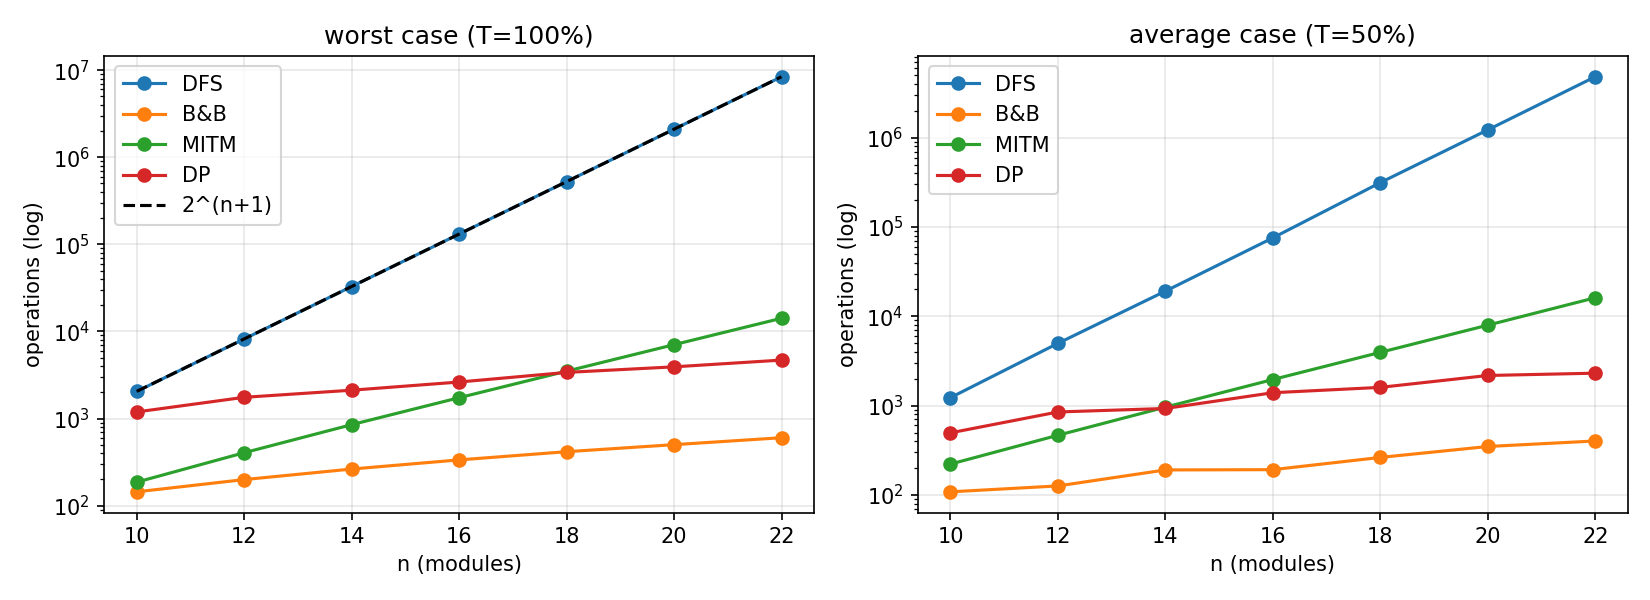
\includegraphics[width=\linewidth]{figures/fig_operations_vs_n.png}\par
{\footnotesize Fonte: elaborado pelos autores (2026).}
\end{minipage}\par\vspace{0.8em}

\textbf{A DP escala.} Custo exatamente n(T+1) em toda instância (como provado): 600 módulos com T=3.060 custam 1.836.600 operações (0,37 s em Python puro). O guloso fica abaixo de 2 ms em qualquer tamanho.

\textbf{Pseudo-polinomialidade na prática.} Mantendo 18 módulos e refinando a unidade de tempo (T de 100 a 102.400), só a DP cresce (1.818 \ensuremath{\rightarrow} 1.843.218 operações); DFS, B\&B, MITM e guloso não mudam: dependem de n e da estrutura da instância, não da magnitude de T.

\textbf{Qualidade da heurística gulosa.} A perda média em relação ao ótimo (\textit{gap}) é pequena e decresce com n (abaixo de 3\% para n\ensuremath{\geq}30, Figura 2), mas o pior caso é severo com poucos módulos: 25,9\% (n=8, \ensuremath{\rho}=0,3), 54,5\% (\ensuremath{\rho}=0,1) e 99,8\% na instância adversarial, formada por dois módulos em que a razão induz a escolha errada. A variante com melhor item corrige apenas os casos em que um módulo sozinho quase preenche a mochila; sua vantagem é a garantia de metade do ótimo, e não a média.

\par\vspace{0.6em}\noindent\begin{minipage}{\linewidth}\singlespacing\centering
{\small Figura 2 -- Perda da heurística gulosa em relação ao ótimo, por orçamento e por número de módulos}\par\vspace{0.3em}
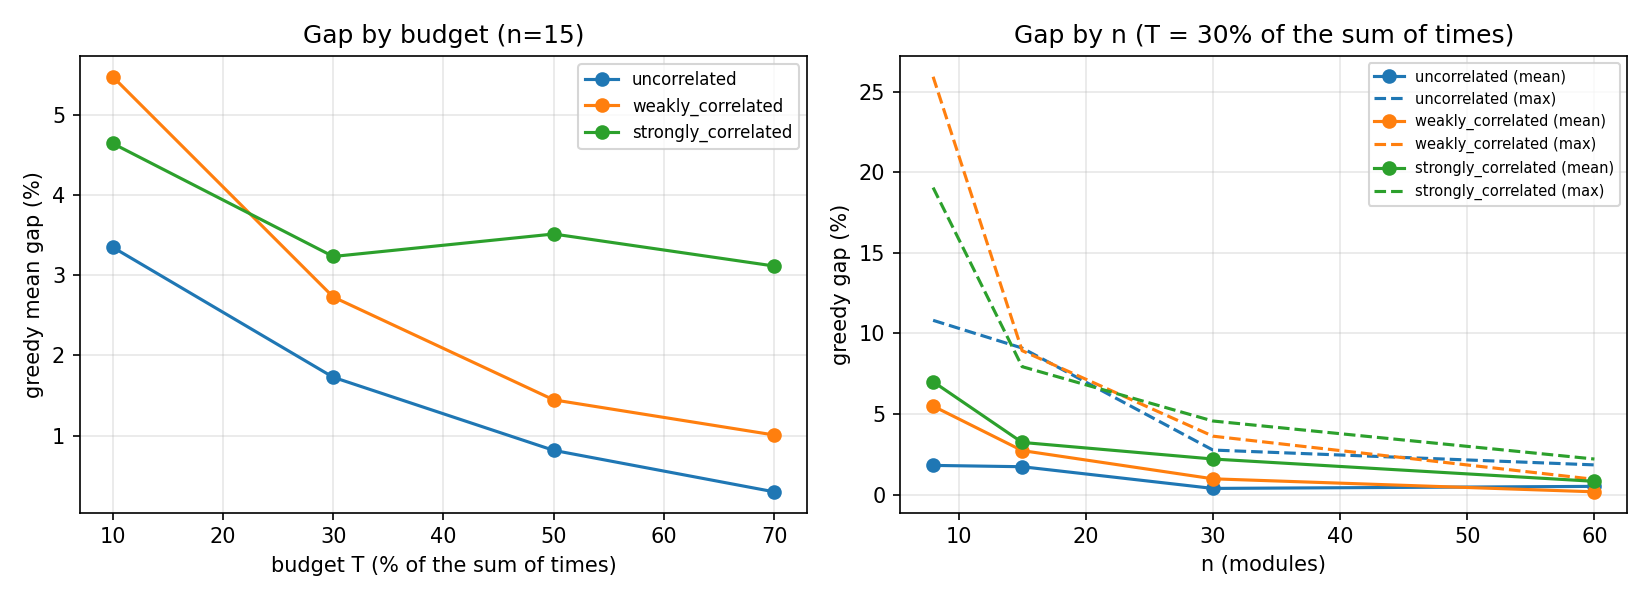
\includegraphics[width=\linewidth]{figures/fig_greedy_quality.png}\par
{\footnotesize Fonte: elaborado pelos autores (2026).}
\end{minipage}\par\vspace{0.8em}

\textbf{B\&B é sensível aos dados; DP e MITM não.} Com R=1000 e n=40, instâncias fortemente correlacionadas custam ao B\&B, em média, 11 a 15\ensuremath{\times} mais que as não correlacionadas (17.162 contra 1.377 operações em n=40); a pior execução chegou a 44.475 operações contra 2.087, cerca de 21\ensuremath{\times}, em linha com a literatura sobre a dificuldade das instâncias da mochila (Pisinger, 2005; Smith-Miles et al., 2021; Jooken et al., 2022). DP e MITM custam idêntico nas duas famílias. O B\&B foi o algoritmo exato mais barato em todas as medições (n\ensuremath{\leq}40), mas é o único cujo custo oscila com os dados e que não tem garantia polinomial. Em instâncias maiores e fortemente correlacionadas, ele pode não terminar em tempo útil (Seção 8).

\textbf{Custo do FPTAS.} Com T pequeno, a aproximação custou de 7,8\ensuremath{\times} a 78\ensuremath{\times} o custo da solução exata com a DP (\ensuremath{\varepsilon} de 0,5 a 0,05). O FPTAS encontrou o ótimo em todos os casos, mas a um custo maior e com garantia mais fraca.

\textbf{A enumeração do RUTICO.} A DFS sobre o grafo de pré-requisitos completo gera exatamente 2\ensuremath{^{n-1}} caminhos (32.768 em n=16): no pior caso, a abordagem do artigo original é exponencial no tamanho do grafo do curso. Grafos de curso reais são mais esparsos, então esse número é um limite superior, e não o caso típico.

\secao{6 VALIDAÇÃO COM DADOS REAIS (PLATAFORMA GuIA / SEBRAE)}
\subsecao{6.1 Extração e anonimização}
Dados extraídos do banco de produção da plataforma por consultas somente de leitura e 100\% agregadas (\textit{job} temporário, destruído após o uso). Nenhum dado pessoal ou texto saiu do banco: cursos e módulos foram convertidos em índices, e os arquivos versionados contêm apenas contagens, medianas e médias. Origem (agregada): 4 cursos, 19 módulos, 86 tópicos, 3.864 matrículas, 576 sessões de módulo com início e fim registrados, 189 notas NPS e 13.573 exercícios corrigidos.

Duas instâncias:

\begin{itemize}[leftmargin=*,itemsep=0.3em]
\item \textbf{Módulos (n=12)}: o tempo é a mediana real observada por módulo (16,5 a 376 min, uma variação de 23\ensuremath{\times} que a carga horária estimada da plataforma, constante em 2h, não captura). Três definições de score: taxa de conclusão (\texttt{conclusao}), n\textsuperscript{o} de tópicos (\texttt{conteudo}) e NPS do curso (\texttt{nps}). Entram os 12 dos 19 módulos que têm tempo medido; os tempos são arredondados para o minuto inteiro mais próximo (mínimo de 1), porque a DP exige tempos inteiros.
\item \textbf{Tópicos (n=78)}: o tempo do módulo é repartido entre os tópicos proporcionalmente ao volume de exercícios de cada um (proxy observado; é uma escolha de modelagem declarada, assim como as definições de score). Scores: nota média dos exercícios (\texttt{dominio}) e n\textsuperscript{o} de tentativas (\texttt{engajamento}). Entram os 78 dos 86 tópicos que têm tempo de módulo e nota média registrados, com o mesmo arredondamento.
\end{itemize}

\subsecao{6.2 O que os dados reais mostraram}
\textbf{Posição dos dados reais entre as famílias sintéticas.} Medimos a correlação de Pearson entre tempo e score (r = +1 indica que crescem juntos, 0 indica ausência de relação e \ensuremath{-}1 indica relação inversa), conforme a Tabela 1.

\par\vspace{0.6em}\noindent\begin{minipage}{\linewidth}\singlespacing
\legenda{Tabela 1 -- Correlação de Pearson entre tempo e score nas instâncias reais}
\small\noindent\begin{tabularx}{\linewidth}{@{}L{1.176}L{0.392}L{0.471}L{1.961}@{}}\toprule
\textbf{Instância / score} & \textbf{n} & \textbf{r} & \textbf{Leitura}\\\midrule
módulos / conteúdo & 12 & \textbf{+0,92} & confirma a hipótese: módulo longo vale mais\\
módulos / conclusão & 12 & \textbf{\ensuremath{-}0,62} & módulo longo conclui menos; regime que nenhuma família sintética cobre\\
módulos / NPS & 12 & \ensuremath{-}0,05 & sem relação\\
tópicos / domínio & 78 & +0,13 & quase sem relação\\
tópicos / engajamento & 78 & +0,29 & relação fraca\\
\bottomrule\end{tabularx}
\fonte{Fonte: elaborado pelos autores (2026).}
\end{minipage}\par\vspace{0.8em}

Há dois resultados: (i) a hipótese do artigo, de que dados de \textit{e-learning} são correlacionados, se confirmou na definição de score por conteúdo, r=+0,92, próximo da família \textit{weakly correlated} (r=0,98 em uma instância sintética de mesmo n) e abaixo da \textit{strongly correlated} (r=1,00); (ii) observação: o score de conclusão produz correlação \textit{negativa}, um regime que as três famílias sintéticas deste trabalho não cobrem. Com n=12, essa estimativa deve ser lida com cautela.

\textbf{Concordância dos exatos e perda do guloso com orçamento curto.} Nas 12 combinações (3 scores \ensuremath{\times} 4 orçamentos), todos os algoritmos exatos acharam a mesma trilha ótima. O guloso perdeu até 21\% com orçamento apertado: 21,0\% com 30 min e 17,3\% com 1h (score de conclusão), e 18,8\% com 1h30 (score de conteúdo). Com 20h a perda foi zero nos três scores. No nível tópico (n=78) o pior gap cai para 7,3\%, o que confirma em dados reais a previsão de que o gap diminui com n.

\textbf{Granularidade: custo e fidelidade.} Repetindo o teste de pseudo-polinomialidade com a instância real (orçamento de 10h): em horas, a DP custa 132 operações; em minutos, 7.212; os demais variam pouco e sem tendência (o B\&B fica entre 124 e 348 operações), porque a mudança de unidade altera os tempos arredondados, mas não o tamanho do problema. Ainda assim, 7.212 operações correspondem a milissegundos. O teste trouxe um resultado adicional: arredondar os tempos para horas mudou a própria resposta ótima (49 pontos em horas contra 56 em minutos, no score de conteúdo). Em horas, a trilha escolhida ocupa só 502 dos 600 minutos reais; em blocos de 15 min, o valor sobe para 57, mas a trilha soma 606 minutos e ultrapassa o orçamento. Uma unidade grossa não traz economia relevante e distorce o problema; a DP com tempos em minutos é barata e mais fiel.

\textbf{Uma execução para todos os orçamentos.} A última linha da tabela da DP entrega o ótimo para \textit{qualquer} orçamento de 0 a 24h de uma só vez, como demonstrado com os dados reais. No produto, isso permite responder qual é a melhor trilha com 2h, 5h ou 10h por semana com uma única execução, em vez de três.

\secao{7 EXPERIMENTO COMPLEMENTAR: METAHEURÍSTICA GRASP}
O MAS-Cloud+ (Mendes et al., 2022), do grupo do Prof. Marotta, provisiona máquinas virtuais na nuvem com três camadas de raciocínio: regras rápidas, metaheurística (GRASP) e otimização formal. Nosso comparativo cobria todas as técnicas menos a metaheurística. O experimento complementar cobre essa lacuna ao adaptar o GRASP (Resende; Ribeiro, 2016) do MAS-Cloud+ ao domínio de trilhas, com semente fixa (reprodutível) e contador de operações como os demais. Metaheurísticas também já foram aplicadas à recomendação de trilhas em MOOCs (Son et al., 2021), o que torna a comparação com o método exato relevante para a área.

\textbf{Validação:} em 1.800 instâncias aleatórias geradas pelo protocolo de correção (três famílias, 40 sementes, cinco valores de \ensuremath{\rho} e n \ensuremath{\in} \{8, 12, 16\}), o GRASP achou o ótimo em 98,1\% dos casos (gap médio 0,044\%, pior 9,4\%). Os gaps do guloso na tabela abaixo vêm das 30 instâncias por célula deste experimento (\ensuremath{\rho}=0,3), com sementes diferentes das da Seção 5; por isso o pior caso em \textit{weakly correlated} com n=8 aparece aqui como 25,0\%, e lá como 25,9\%.

A Tabela 2 compara o guloso e o GRASP nos principais cenários.

\par\vspace{0.6em}\noindent\begin{minipage}{\linewidth}\singlespacing
\legenda{Tabela 2 -- Guloso e GRASP: pior gap e custo relativo}
\small\noindent\begin{tabularx}{\linewidth}{@{}L{1.333}L{0.833}L{0.833}@{}}\toprule
\textbf{Cenário} & \textbf{Guloso} & \textbf{GRASP}\\\midrule
weakly corr., n=8 (pior gap) & 25,0\% & \textbf{0,0\%}\\
real, módulos/conclusão (pior gap) & 21,0\% & \textbf{0,0\%}\\
real, módulos/conteúdo (pior gap) & 18,8\% & 1,5\%\\
instância adversarial & 2 (ótimo: 1000) & \textbf{1000}\\
custo relativo ao guloso & 1\ensuremath{\times} & 50\ensuremath{\times} a 260\ensuremath{\times}\\
\bottomrule\end{tabularx}
\fonte{Fonte: elaborado pelos autores (2026).}
\end{minipage}\par\vspace{0.8em}

\textbf{Comparação com a DP exata:} na instância real de tópicos (n=78), o GRASP custou 4,5\ensuremath{\times} mais que a DP exata (211.950 contra 46.878 operações) e ainda assim perdeu até 3,2\%, mais que o próprio guloso nesse score (2,3\%). No nível de módulos (n=12), o GRASP custou cerca de metade das operações da DP (3.580 contra 7.212), com gap de 0\% a 1,5\%. Nos dois níveis, só a DP garante o ótimo. Esse resultado vai na mesma direção do que o MAS-Cloud+ relata em seu domínio, onde a otimização formal superou a metaheurística em 19,3\% de desempenho com 6,5\% menos custo. Nos dois domínios, quando a instância cabe no método exato, o método exato é a melhor escolha; a metaheurística é a alternativa para quando a instância não cabe, e com o T pequeno das trilhas de estudo esse caso não apareceu em nenhuma instância testada.

\secao{8 VALIDAÇÃO INDEPENDENTE COM BIBLIOTECAS}
Os experimentos anteriores comparam os algoritmos do grupo entre si, de modo que um erro comum a todos passaria despercebido. Para ter uma referência externa, repetimos as verificações com bibliotecas consolidadas: OR-Tools 9.15 (Google, 2026) e SciPy 1.18 (Virtanen et al., 2020), esta com o solver HiGHS de programação inteira, como oráculos do valor ótimo; NumPy 2.5 (Harris et al., 2020) e SciPy para a correlação de Pearson; e a função \texttt{sorted} do Python para a ordenação. O script \texttt{experiment\_validation.py} reproduz todos os resultados desta seção.

\textbf{Valor ótimo.} Em 3.533 instâncias, nenhum algoritmo exato do grupo divergiu das bibliotecas (Tabela 3), e as duas bibliotecas concordaram entre si em todas. Com a tolerância padrão, o HiGHS parou a 1 ponto do ótimo em 5 instâncias de tópicos; com tolerância zero (\texttt{mip\_rel\_gap=0}), a diferença desapareceu.

\par\vspace{0.6em}\noindent\begin{minipage}{\linewidth}\singlespacing
\legenda{Tabela 3 -- Divergências entre os algoritmos exatos do grupo e as bibliotecas de referência}
\small\noindent\begin{tabularx}{\linewidth}{@{}L{1.308}L{0.598}L{1.495}L{0.598}@{}}\toprule
\textbf{Conjunto} & \textbf{Instâncias} & \textbf{Algoritmos do grupo verificados} & \textbf{Divergências}\\\midrule
Protocolo de correção (n\ensuremath{\leq}16) & 1.200 & DP (três variantes), DFS, B\&B, MITM & 0\\
Protocolo do GRASP (n\ensuremath{\leq}16) & 1.800 & DP (três variantes), DFS, B\&B, MITM & 0\\
Sintéticas grandes (n=50 a 600) & 90 & DP (três variantes) & 0\\
Reais, módulos (n=12) & 285 & DP (três variantes), DFS, B\&B, MITM & 0\\
Reais, tópicos (n=78) & 158 & DP (três variantes), B\&B & 0\\
\textbf{Total} & \textbf{3.533} &  & \textbf{0}\\
\bottomrule\end{tabularx}
\fonte{Fonte: elaborado pelos autores (2026).}
\end{minipage}\par\vspace{0.8em}

\textbf{Garantias e GRASP.} Medidas contra o ótimo do OR-Tools, as garantias do guloso com melhor item (pelo menos metade do ótimo) e do FPTAS (pelo menos 90\% do ótimo com \ensuremath{\varepsilon}=0,1) valeram nas 1.200 instâncias do protocolo de correção. Os resultados do GRASP se repetiram: ótimo em 98,1\% das 1.800 instâncias, gap médio de 0,044\% e pior gap de 9,4\%.

\textbf{Ordenação e correlação.} O \textit{merge sort} do grupo produziu a mesma ordem que a função \texttt{sorted}, com chaves racionais exatas, em 1.295 listas. As três implementações da correlação de Pearson diferem apenas a partir da 16\textsuperscript{a} casa decimal. O SciPy fornece ainda a significância: no score de conclusão, r=\ensuremath{-}0,62 tem p=0,03 e intervalo de confiança de 95\% entre \ensuremath{-}0,88 e \ensuremath{-}0,08; no score de conteúdo, r=+0,92 tem intervalo entre +0,73 e +0,98; no score de engajamento, r=+0,29 tem p=0,01. As correlações dos scores de NPS (p=0,89) e de domínio (p=0,25) não são significativas.

\textbf{Tempo de execução.} A DP em Python puro é mais lenta que as bibliotecas compiladas: de 13,5 vezes (n=50) a 3,3 vezes (n=600) em relação ao OR-Tools, que para n>40 também usa programação dinâmica, e 28 vezes em relação ao HiGHS em n=600 (206 ms contra 7,4 ms), segundo os tempos registrados em \texttt{results/validation\_runtime.csv}. Tempos de relógio variam entre execuções e máquinas; a comparação por contadores de operações não é afetada por essa diferença.

\textbf{Limite do B\&B.} A validação mostrou um comportamento que os experimentos até n=40 não revelavam: em instâncias fortemente correlacionadas com \ensuremath{\rho}=0,5 e limite de 20 s por execução, o B\&B do grupo não terminou em 7 de 15 execuções (as três de n=600, duas de três em n=400 e duas de três em n=200), enquanto a DP resolveu cada uma em até 0,2 s.

\secao{9 DISCUSSÃO: ESCOLHA DO ALGORITMO}
O Quadro 3 resume a escolha de algoritmo conforme a situação.

\par\vspace{0.6em}\noindent\begin{minipage}{\linewidth}\singlespacing
\legenda{Quadro 3 -- Escolha de algoritmo conforme a situação}
\small\noindent\begin{tabularx}{\linewidth}{@{}L{1.111}L{0.889}@{}}\toprule
\textbf{Situação} & \textbf{Escolha}\\\midrule
T inteiro pequeno (minutos de estudo), n até milhares, precisa de garantia & \textbf{Programação dinâmica}\\
Resposta instantânea, muitos módulos pequenos, perda de 1--3\% aceitável & Guloso + melhor item\\
T gigante (unidade finíssima), n \ensuremath{\lesssim} 40 & Meet-in-the-Middle\\
n grande demais para os exatos, sem garantia exigida & GRASP (complementar)\\
Instâncias fáceis, n moderado, velocidade média importa mais & Branch and Bound\\
n e T gigantes, erro \ensuremath{\varepsilon} tolerável & FPTAS\\
Pré-requisitos (ordem) & enumeração como no RUTICO, programação inteira (Aslan et al., 2023) ou DP em árvore\\
Tempos incertos & mochila com restrições probabilísticas (Aslan et al., 2023)\\
\bottomrule\end{tabularx}
\fonte{Fonte: elaborado pelos autores (2026).}
\end{minipage}\par\vspace{0.8em}

A recomendação do trabalho é a DP, por cinco razões sustentadas pelos experimentos sintéticos e reais: (1) é exata, e o guloso demonstrou perder até 21\% com o aluno de pouco tempo; (2) o parâmetro que a encarece (T) é pequeno neste domínio, e com tempos em minutos a execução leva milissegundos; (3) o custo é previsível, com exatamente n(T+1) operações conhecidas antes da execução, enquanto o B\&B oscilou 11--15\ensuremath{\times} entre famílias e não terminou em 20 s em 7 de 15 instâncias grandes fortemente correlacionadas (Seção 8), e o GRASP não oferece garantia; (4) o custo da DP não muda com a correlação dos dados, que nas instâncias reais variou de r=\ensuremath{-}0,62 a r=+0,92, enquanto o B\&B se mostrou sensível a ela nos experimentos sintéticos; (5) uma tabela responde todos os orçamentos de uma vez.

Em relação à literatura recente (Seção 3), essa recomendação ocupa um espaço próprio: os métodos de recomendação de trilhas baseados em grafos de conhecimento, aprendizado por reforço ou LLMs ordenam e personalizam, mas não garantem o ótimo da seleção sob orçamento; a DP garante esse ótimo com custo previsível e pode ser combinada com eles, escolhendo o conjunto de módulos antes da ordenação.

\secao{10 LIMITAÇÕES}
Os resultados devem ser lidos com as limitações a seguir.

\textbf{Relaxação do problema.} O modelo ignora pré-requisitos e ordem de estudo, que o RUTICO trata no grafo do curso. As conclusões valem para a escolha entre módulos independentes; com precedência, o problema passa a ser a mochila com precedência, à qual a DP aqui apresentada não se aplica diretamente. Aslan et al. (2023) tratam esse caso mais geral em sistemas de aprendizagem personalizada.

\textbf{Tamanho das instâncias reais.} A instância de módulos tem n=12 e a de tópicos tem n=78, extraídas de uma única plataforma. As correlações medidas, em especial r=\ensuremath{-}0,62 no score de conclusão, têm incerteza alta (intervalo de confiança de 95\% entre \ensuremath{-}0,88 e \ensuremath{-}0,08, Seção 8) e não devem ser generalizadas para outros catálogos.

\textbf{Scores e tempos aproximados.} Taxa de conclusão, número de tópicos, NPS, nota média e número de tentativas aproximam o valor de um módulo, mas não medem aprendizagem. O NPS é medido por curso, o que deixa apenas três valores distintos entre os 12 módulos. O tempo de cada tópico vem do rateio do tempo do módulo pelo volume de exercícios, e o score de engajamento também deriva dos exercícios, o que pode elevar a correlação entre os dois. Além disso, o modelo usa a mediana como tempo fixo de cada módulo; a variabilidade entre alunos poderia ser tratada com estimativas de incerteza, como em Nabizadeh et al. (2019), ou com restrições probabilísticas, como em Aslan et al. (2023).

\textbf{Arredondamento.} Os tempos medianos foram arredondados para o minuto inteiro mais próximo, de modo que o tempo de uma trilha pode diferir do tempo real em até meio minuto por módulo.

\textbf{Medição de custo.} Os contadores de operações não dependem da máquina, mas contam unidades diferentes em cada algoritmo, e os tempos de relógio vêm de uma única máquina e de um único interpretador. Os algoritmos exponenciais foram medidos até n=22 (DFS) e n=40 (B\&B e MITM) nos experimentos principais; além desses tamanhos, o comportamento foi obtido por prova e extrapolação, e apenas o B\&B foi levado até n=600, na validação da Seção 8.

\secao{11 CONCLUSÃO}
Modelamos a seleção de módulos sob orçamento de tempo como o problema da mochila 0/1 e mostramos que, no problema relaxado sem pré-requisitos, a programação dinâmica é a enumeração exaustiva do RUTICO com memória: as 2\ensuremath{^{n}} folhas da árvore de decisão colapsam em n(T+1) estados. Provamos a correção e os limites de custo de todos os algoritmos, medimos o custo com contadores de operações independentes de máquina, conferimos os resultados com bibliotecas externas e levamos a comparação a dados reais de uma plataforma em produção, que confirmaram a hipótese de correlação, mostraram um regime negativamente correlacionado que as famílias sintéticas testadas não cobrem e mostraram o guloso falhando no perfil de aluno com pouco tempo. O experimento complementar com o GRASP cobriu a técnica que faltava e, ao ficar mais caro e menos preciso que a DP na instância de tópicos, chegou em \textit{e-learning} a uma conclusão alinhada à do MAS-Cloud+ na nuvem: quando o problema cabe no método exato, ele é a melhor escolha.

A comparação com a literatura recente mostra que a recomendação de trilhas avançou sobretudo em modelos de aprendizado (grafos de conhecimento, aprendizado por reforço e LLMs), que priorizam a ordem e a personalização, sem garantia de ótimo. A seleção exata sob orçamento estudada aqui é complementar a essas abordagens.

\textbf{Trabalhos futuros.} Reintroduzir os pré-requisitos (mochila com precedência, NP-difícil em DAGs gerais, mas com DP viável em árvores), partindo do modelo de Aslan et al. (2023), que também trata a incerteza dos tempos; restrições múltiplas (tempo + custo computacional de LLM, uma mochila multidimensional, como a formulada por Tsamis et al. (2025) para recursos educacionais, com aplicação direta na plataforma real: rotear interações do aluno para modelos de linguagem de capacidades e custos diferentes conforme a necessidade, nos moldes do próprio MAS-Cloud+); combinar a seleção exata com métodos de sequenciamento (Chen et al., 2023; Li et al., 2023); e instâncias maiores em linguagem compilada.

\clearpage
\begin{center}{\bfseries REFERÊNCIAS}\end{center}\vspace{0.5em}
\begin{singlespace}\raggedright
\noindent ASLAN, Ayse; URSAVAS, Evrim; ROMEIJNDERS, Ward. A precedence constrained knapsack problem with uncertain item weights for personalized learning systems. \textbf{Omega}, v. 115, 102779, 2023. DOI: 10.1016/j.omega.2022.102779.\par\vspace{1em}
\noindent CACCHIANI, Valentina; IORI, Manuel; LOCATELLI, Alberto; MARTELLO, Silvano. Knapsack problems --- an overview of recent advances. Part I: single knapsack problems. \textbf{Computers \& Operations Research}, v. 143, 105692, 2022. DOI: 10.1016/j.cor.2021.105692.\par\vspace{1em}
\noindent CHEN, Xianyu et al. Set-to-sequence ranking-based concept-aware learning path recommendation. \textbf{Proceedings of the AAAI Conference on Artificial Intelligence}, v. 37, n. 4, p. 5027-5035, 2023. DOI: 10.1609/aaai.v37i4.25630.\par\vspace{1em}
\noindent DANTZIG, George B. Discrete-variable extremum problems. \textbf{Operations Research}, v. 5, n. 2, p. 266-288, 1957.\par\vspace{1em}
\noindent GOOGLE. \textbf{OR-Tools}. Versão 9.15. [S. l.]: Google, 2026. Disponível em: https://developers.google.com/optimization. Acesso em: 15 nov. 2026.\par\vspace{1em}
\noindent HARRIS, Charles R. et al. Array programming with NumPy. \textbf{Nature}, v. 585, p. 357-362, 2020.\par\vspace{1em}
\noindent JOOKEN, Jorik; LEYMAN, Pieter; DE CAUSMAECKER, Patrick. A new class of hard problem instances for the 0-1 knapsack problem. \textbf{European Journal of Operational Research}, v. 301, n. 3, p. 841-854, 2022. DOI: 10.1016/j.ejor.2021.12.009.\par\vspace{1em}
\noindent LI, Qingyao et al. Graph enhanced hierarchical reinforcement learning for goal-oriented learning path recommendation. In: ACM INTERNATIONAL CONFERENCE ON INFORMATION AND KNOWLEDGE MANAGEMENT, 32., 2023, Birmingham. \textbf{Proceedings} [...]. New York: ACM, 2023. p. 1318-1327. DOI: 10.1145/3583780.3614897.\par\vspace{1em}
\noindent LV, Rui et al. GenAL: generative agent for adaptive learning. \textbf{Proceedings of the AAAI Conference on Artificial Intelligence}, v. 39, n. 1, p. 577-585, 2025. DOI: 10.1609/aaai.v39i1.32038.\par\vspace{1em}
\noindent MENDES, Aldo H. D. et al. \textbf{MAS-Cloud+}: a multiagent architecture for optimized cloud resource management. SSRN, 2022. Preprint. DOI: 10.2139/ssrn.4059930.\par\vspace{1em}
\noindent NABIZADEH, Amir Hossein; JORGE, Alípio Mário; LEAL, José Paulo. RUTICO: recommending successful learning paths under time constraints. In: CONFERENCE ON USER MODELING, ADAPTATION AND PERSONALIZATION, 25., 2017, Bratislava. \textbf{Adjunct Publication} [...]. New York: ACM, 2017. DOI: 10.1145/3099023.3099035.\par\vspace{1em}
\noindent NABIZADEH, Amir Hossein; JORGE, Alípio Mário; LEAL, José Paulo. Estimating time and score uncertainty in generating successful learning paths under time constraints. \textbf{Expert Systems}, v. 36, n. 2, e12351, 2019. DOI: 10.1111/exsy.12351.\par\vspace{1em}
\noindent NABIZADEH, Amir Hossein et al. Adaptive learning path recommender approach using auxiliary learning objects. \textbf{Computers \& Education}, v. 147, 103777, 2020a. DOI: 10.1016/j.compedu.2019.103777.\par\vspace{1em}
\noindent NABIZADEH, Amir Hossein et al. Learning path personalization and recommendation methods: a survey of the state-of-the-art. \textbf{Expert Systems with Applications}, v. 159, 113596, 2020b. DOI: 10.1016/j.eswa.2020.113596.\par\vspace{1em}
\noindent PISINGER, David. Where are the hard knapsack problems? \textbf{Computers \& Operations Research}, v. 32, n. 9, p. 2271-2284, 2005.\par\vspace{1em}
\noindent RAHAYU, Nur W.; FERDIANA, Ridi; KUSUMAWARDANI, Sri S. A systematic review of learning path recommender systems. \textbf{Education and Information Technologies}, v. 28, n. 6, p. 7437-7460, 2023. DOI: 10.1007/s10639-022-11460-3.\par\vspace{1em}
\noindent RESENDE, Mauricio G. C.; RIBEIRO, Celso C. \textbf{Optimization by GRASP}: greedy randomized adaptive search procedures. New York: Springer, 2016. DOI: 10.1007/978-1-4939-6530-4.\par\vspace{1em}
\noindent SHI, Daqian; WANG, Ting; XING, Hao; XU, Hao. A learning path recommendation model based on a multidimensional knowledge graph framework for e-learning. \textbf{Knowledge-Based Systems}, v. 195, 105618, 2020. DOI: 10.1016/j.knosys.2020.105618.\par\vspace{1em}
\noindent SMITH-MILES, Kate; CHRISTIANSEN, Jeffrey; MUÑOZ, Mario Andrés. Revisiting where are the hard knapsack problems? via instance space analysis. \textbf{Computers \& Operations Research}, v. 128, 105184, 2021. DOI: 10.1016/j.cor.2020.105184.\par\vspace{1em}
\noindent SON, Ngo Tung; JAAFAR, Jafreezal; AZIZ, Izzatdin Abdul; ANH, Bui Ngoc. Meta-heuristic algorithms for learning path recommender at MOOC. \textbf{IEEE Access}, v. 9, p. 59093-59107, 2021. DOI: 10.1109/ACCESS.2021.3072222.\par\vspace{1em}
\noindent TSAMIS, George et al. A multi-constrained knapsack approach for educational resource allocation: genetic algorithm with category-specific optimization. \textbf{Electronics}, v. 14, n. 19, 3898, 2025. DOI: 10.3390/electronics14193898.\par\vspace{1em}
\noindent VIRTANEN, Pauli et al. SciPy 1.0: fundamental algorithms for scientific computing in Python. \textbf{Nature Methods}, v. 17, p. 261-272, 2020.\par\vspace{1em}
\end{singlespace}
\clearpage
\begin{center}{\bfseries APÊNDICE A -- DIVISÃO DE ATIVIDADES}\end{center}\vspace{0.5em}
Conforme o artigo: estudo do RUTICO e DFS; DP, provas e instância de teste; guloso, ordenação e algoritmos extras; experimentos, gráficos e escrita. Todos os membros revisaram o código e o texto integralmente e respondem por qualquer parte.

\clearpage
\begin{center}{\bfseries APÊNDICE B -- REPRODUÇÃO DOS EXPERIMENTOS}\end{center}\vspace{0.5em}
Os experimentos são reproduzidos com os comandos a seguir, executados na raiz do repositório.

\begin{singlespace}\small
\begin{verbatim}
python experiment.py             # experimentos sintéticos (branch main)
python experiment_validation.py  # validação com bibliotecas (branch main;
                                 #   requer ortools, scipy e numpy)
python experiment_real.py        # instâncias reais (branch real-data-guia)
python experiment_grasp.py       # experimento complementar GRASP
                                 #   (branch real-data-guia)
\end{verbatim}
\end{singlespace}
As saídas ficam em \texttt{results/*.csv}. Os dados reais anonimizados estão em \texttt{real\_data/}; reproduzir os experimentos não exige acesso à infraestrutura do Sebrae. O branch \texttt{main} contém os algoritmos (inclusive o GRASP), os experimentos sintéticos, as instâncias reais (\texttt{real\_instances.py}) e a validação com bibliotecas; os scripts \texttt{experiment\_real.py} e \texttt{experiment\_grasp.py} estão no branch \texttt{real-data-guia}.

\end{document}
